\chapter{Introduction \& Background}
Alright, so the thing that is on everybody's mind is probably: what is an atomic
swap? An atomic swap is where two parties exchange assets atomically, which means
that either the transaction takes place fully, or the state is reset to the pre-
exchange state.

*Read from oracle defenition*

This is made possible by clever use of cryptography and
programmable contracts on the bitcoin network and blockchain. So before we can
go into more detail on this I should first cover the basics of Bitcoin.

So, most people, especially in computer science, have heard of Bitcoin, but I could
almost count on one hand the number of people I have met that have more than
a basic understanding of how it works. I could talk for hours about this
subject, but sadly there is no time for that. So I will try to give you the
shortest possible version where you can at least understand the rest of my
thesis.

The simplest description of Bitcoin is a shared public ledger, that relies
on proof-of-work to build network-wide consensus. First of proof-of-work
is a way to prove mathematically that work was put into doing something.
The most common way of doing this is via hashing of some datatype.
The hash has to meet certain criteria to be accepted. There is no known
way of producing a wanted hash, so the only way is to try different combinations
until a good result is found. So if you have data that produces a certain hash
that hash serves as proof that you put work into creating it.

Another thing you have probably heard about before is the blockchain, but
just as with Bitcoin overall, people know little about what it actually is.
A blockchain is basically a shared datatype. It is very reminiscent of a
linked list, but allows for branching, meaning that two elements can link
to the same parent. We will come back to this in a moment, but first, let's
take a closer look at the blocks.

A block is a data structure that has a header and data. The header contains
metadata about the block itself as well as a reference to the previous block
in the chain. In Bitcoins case, the data in the block is just a list of transactions,
but you could put anything you want into this field. The reference to the previous
block is what forms the chain. You can from any block follow the references
all the way back to the original block. Anyone can add a block to the chain. But
it has to meet the proof-of-work criteria. The Bitcoin network independently calculates
something called mining-difficulty. This is represented by a large 256-bit number.
For your new block to be accepted the header of the block has to produce a hash that
is strictly smaller than the difficulty number. You produce unique hashes by changing
a field in the header called nonce, this process is what is referred to as mining.

The mining-difficulty is set so that the sum of all participant's hash-calculating power,
or hashrate, will produce  new block on average every 10 minutes. The difficulty is adjusted
every 2016th block.

So how does proof-of-work ensure that the shared ledger stays consistent? This is
where concepts like longest chain comes in. The Bitcoin network only accepts the longest
chain as truth, in other words the chain with most accumulated proof-of-work.
This works as long as the majority of participants is honest. However due to the
probabilistic manner of how new valid blocks are found there is still a chance for
contention even if all participants are honest. For example what will the network do
in the case where two different blocks are found at almost the same time, in
different parts of the network? Now
there are two chains of equal length. So how does the network decide which one
is correct?

*Explain pictures*

\Subsection{Elliptic curve cryptography}
For cryptographic purposes Bitcoin uses a elliptic curve, known simply as elliptic curve 
cryptography or shortend ecc. I will not cover the exact details of the maths, it can 
be found in details in my report, basically all you need to know is that it is an
assymmetric cryptography, meaning it has private and public keys.
 
Though encryption and decryption is possible with ecc it is not the purpose it serves 
for Bitcoin. What is used is signing. This is a concept that all computer scientists
should be familiar with but basically what it means is that you can sign a string
of data with a private key, and that signature could be independently verified by someone who
has the data prior to signing and the public key belonging to the private key, all
without revealing the private key.

Clasically signing is used to prove identity. For example a website could sign
a document to prove that it truly was sent by the server it purports to be.
This is a very useful feature, but in the world of smart contracts the signature
has more significance.

Signatures tend to hold the following significance:

* \textbf{Identity} - A signatures serves as proof that it came from the holder
of the private key. 

* \textbf{Immutability} - A signature makes whatever was signed immutable in a way.
If the data is manipulated after the signing the signature will no longer be valid.

* \textbf{Agreement} - A signature can serve as proof that the holder of a private 
key agreed or approved to whatever data was signed. For example signing a digital
contract could be seen as agreement to the conditions in the contract. The agreement
can't be withdrawn at a later date as the signature proves mathematically that you 
signed it. There is of course the possibility that the private key was stolen. Just
goes to show how important it is to keep the private key private, especially in
Bitocin.

Keep the 3 above points in mind. As they are absolutley vital for the functionality 
of smart contracts.   

%https://en.bitcoin.it/wiki/Transaction
%mastering bitcoin
\Section{Transactions}\label{transactions}
Transactions in Bitcoin are not as straight forward as you might expect a transaction to be. A transaction contains a list of inputs and a list of outputs as well as some metadata like version number and lock-time.\cite{bitcoin_core_tx}\cite{antonopoulos_2017}

\begin{figure}[H]
	\centering
	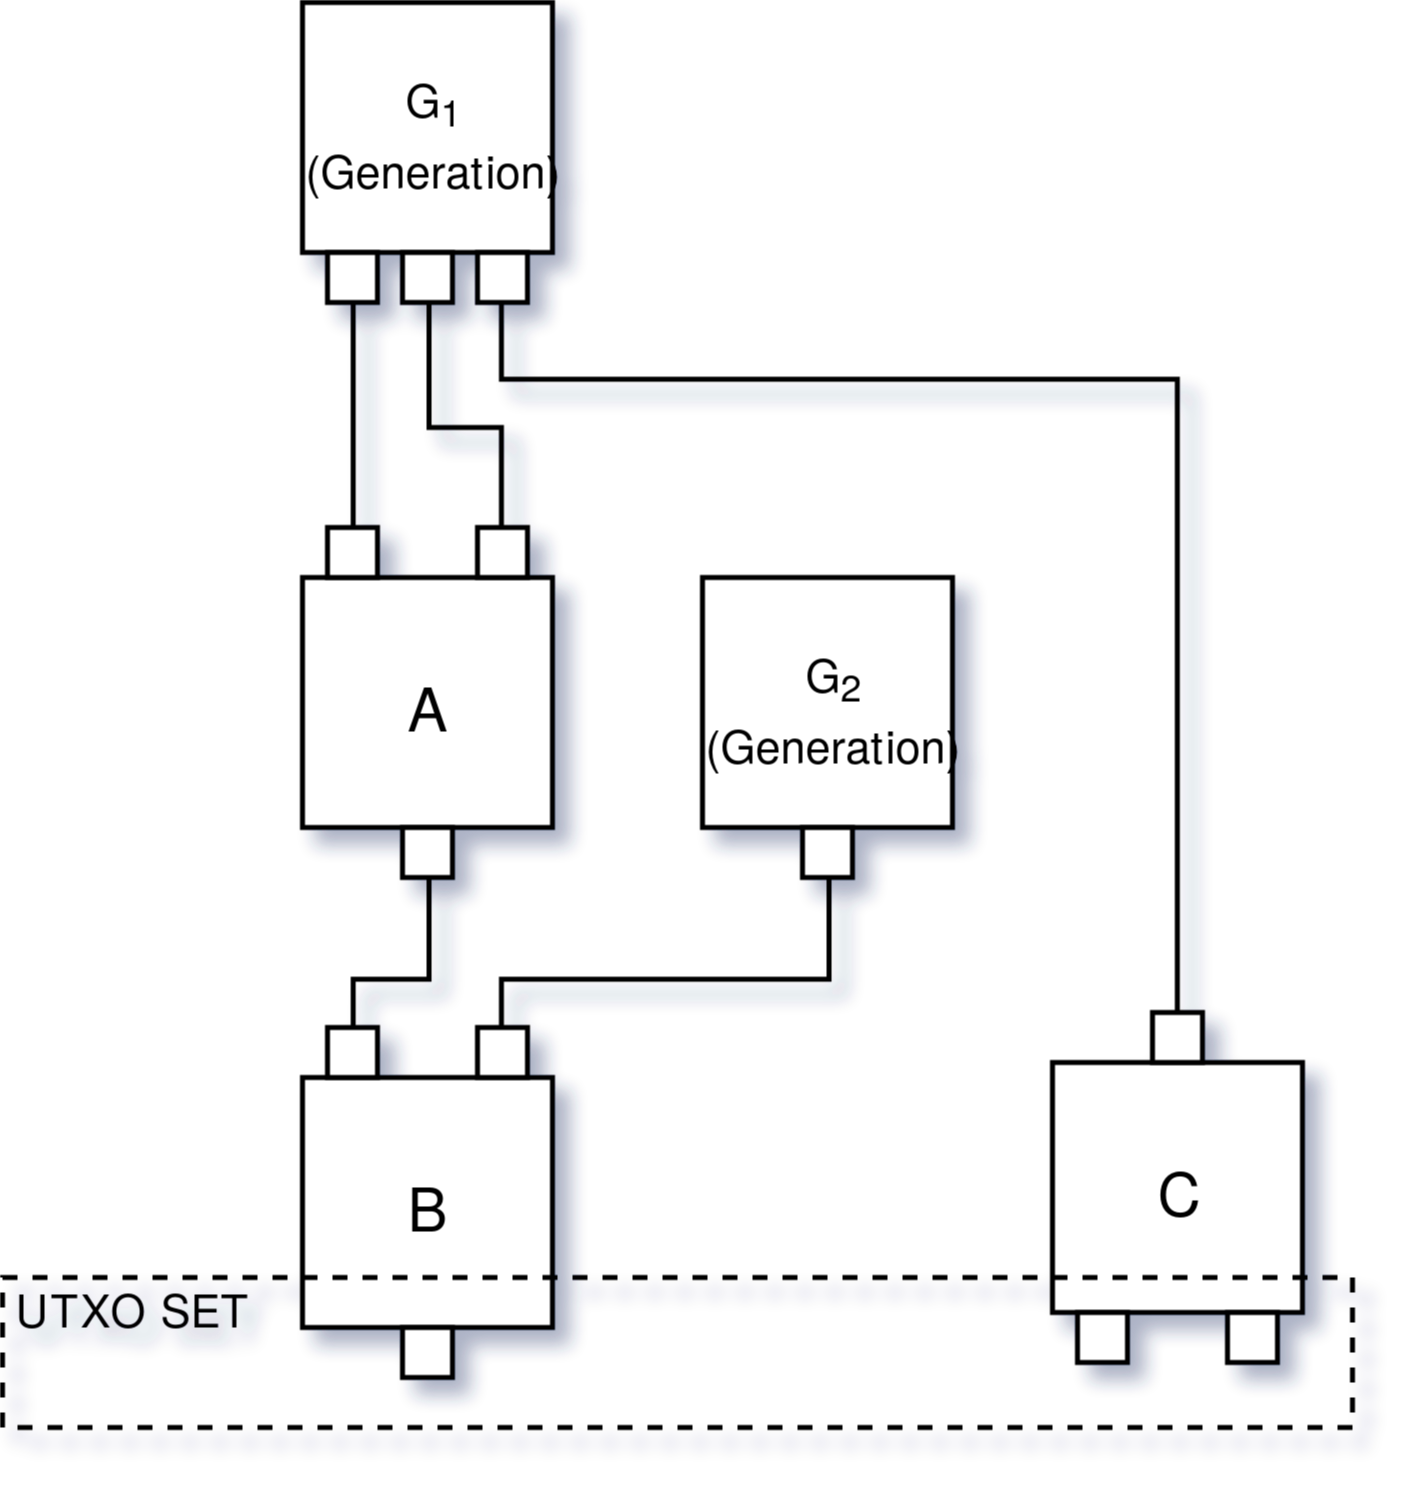
\includegraphics[width=0.75\textwidth]{background/images/transaction_diagram.png}
	\caption{4 example transactions and how inputs are connected to outputs}
	\label{fig:transaction_input_output}
\end{figure}

In simplified terms an output could be seen as the destination of a transaction, in other words it says how much and to whom the transaction is sent to. An input is a reference to a previous output. The inputs take the money from the outputs they reference and that money is used to fund the new outputs.\cite{antonopoulos_2017}\cite{bitcoin_core_tx}

The inputs and outputs is where Script comes into the picture. Both outputs and inputs contains an incomplete script, together however they complete the script. The script in an output could be seen as a challenge, and the script in the input is the response. When a transaction is tested for validity the input script is appended to the script in the output and is executed. If the script comes out as valid the transaction is also valid.\cite{antonopoulos_2017}\cite{bitcoin_core_tx} Here is a basic example: Let's say Alice wants to send a transaction to whoever can answer the equation $4+3$. Her transaction output would contain the script:

\texttt{4 3 OP\_ADD OP\_EQUALS}

If this is executed as is it is invalid. But let's say Bob knows the answer to the equation he can then create a new transaction where the input contains the script: 

\texttt{7} 

Just as before this script is not valid by itself. But then the transaction is checked for validity the input will be appended to the start of the output script forming the following: 

\texttt{7 4 3 OP\_ADD OP\_EQUALS}

Which is a valid script, thus Bobs new transaction is also valid and he may spend the money as he see fits. 

Obviously most transactions on the Bitcoin blockchain are not this simple. The most common form of transaction contains a script called P2PKH which stands for Pay to public key hash. Before we can go into details on this one however we first need to know about how signatures and sighash work in script and transactions.

\Subsection{Signatures and sighash}
Section \ref{ecdsa} covers public keys and signatures in depth.

Perhaps the most important operation in script is the \texttt{OP\_CHECKSIG} operation and its cousins. \texttt{OP\_CHECKSIG} pops two values from the stack, if the script is correctly implemented these two values should be the public key and a signature created with the private key that correlates with mentioned public key

The question is: what is signed when the signature is created? Broadly speaking it is the hash of the transaction that is trying to spend the output, this is not entirely accurate however.\cite{antonopoulos_2017} Appended to the signature that is a flag called \textbf{sighash} (Signature hash). The value of sighash tells the script interpreter what hash was signed during the creation of the signature.\cite{bitcoin_core_sighash} There are 4 types of sighash implemented:

\Subsubsection{SIGHASH\_ALL}
This can be considered the default sighash, if it is not stated otherwise it can safely be assumed that this type was used. This simply means that the entire transaction is signed with all outputs and all other inputs.

\Subsubsection{SIGHASH\_NONE}
This one signs the transaction but without the outputs, it could be thought of as ''I don't care where the money goes''.

\Subsubsection{SIGHASH\_SINGLE}
All outputs are removed except the output with the same index as the input that is being signed, then that transaction is signed.
This could be thought of as ''I dont care about any other outputs to this transaction as long as this one remains as is''.

\Subsubsection{SIGHASH\_ANYONECANPAY}
Signs the transaction with all the outputs but none of the other inputs. This basically means ''The money has to go here, but I don't care if someone else want to fund this transaction also''

%\Subsubsection{More detailed process}
%On the next page the entire signing process for SIGHASH\_ALL is detailed. This is how it is performed in the actual implementation:
%\newpage
%\centerline{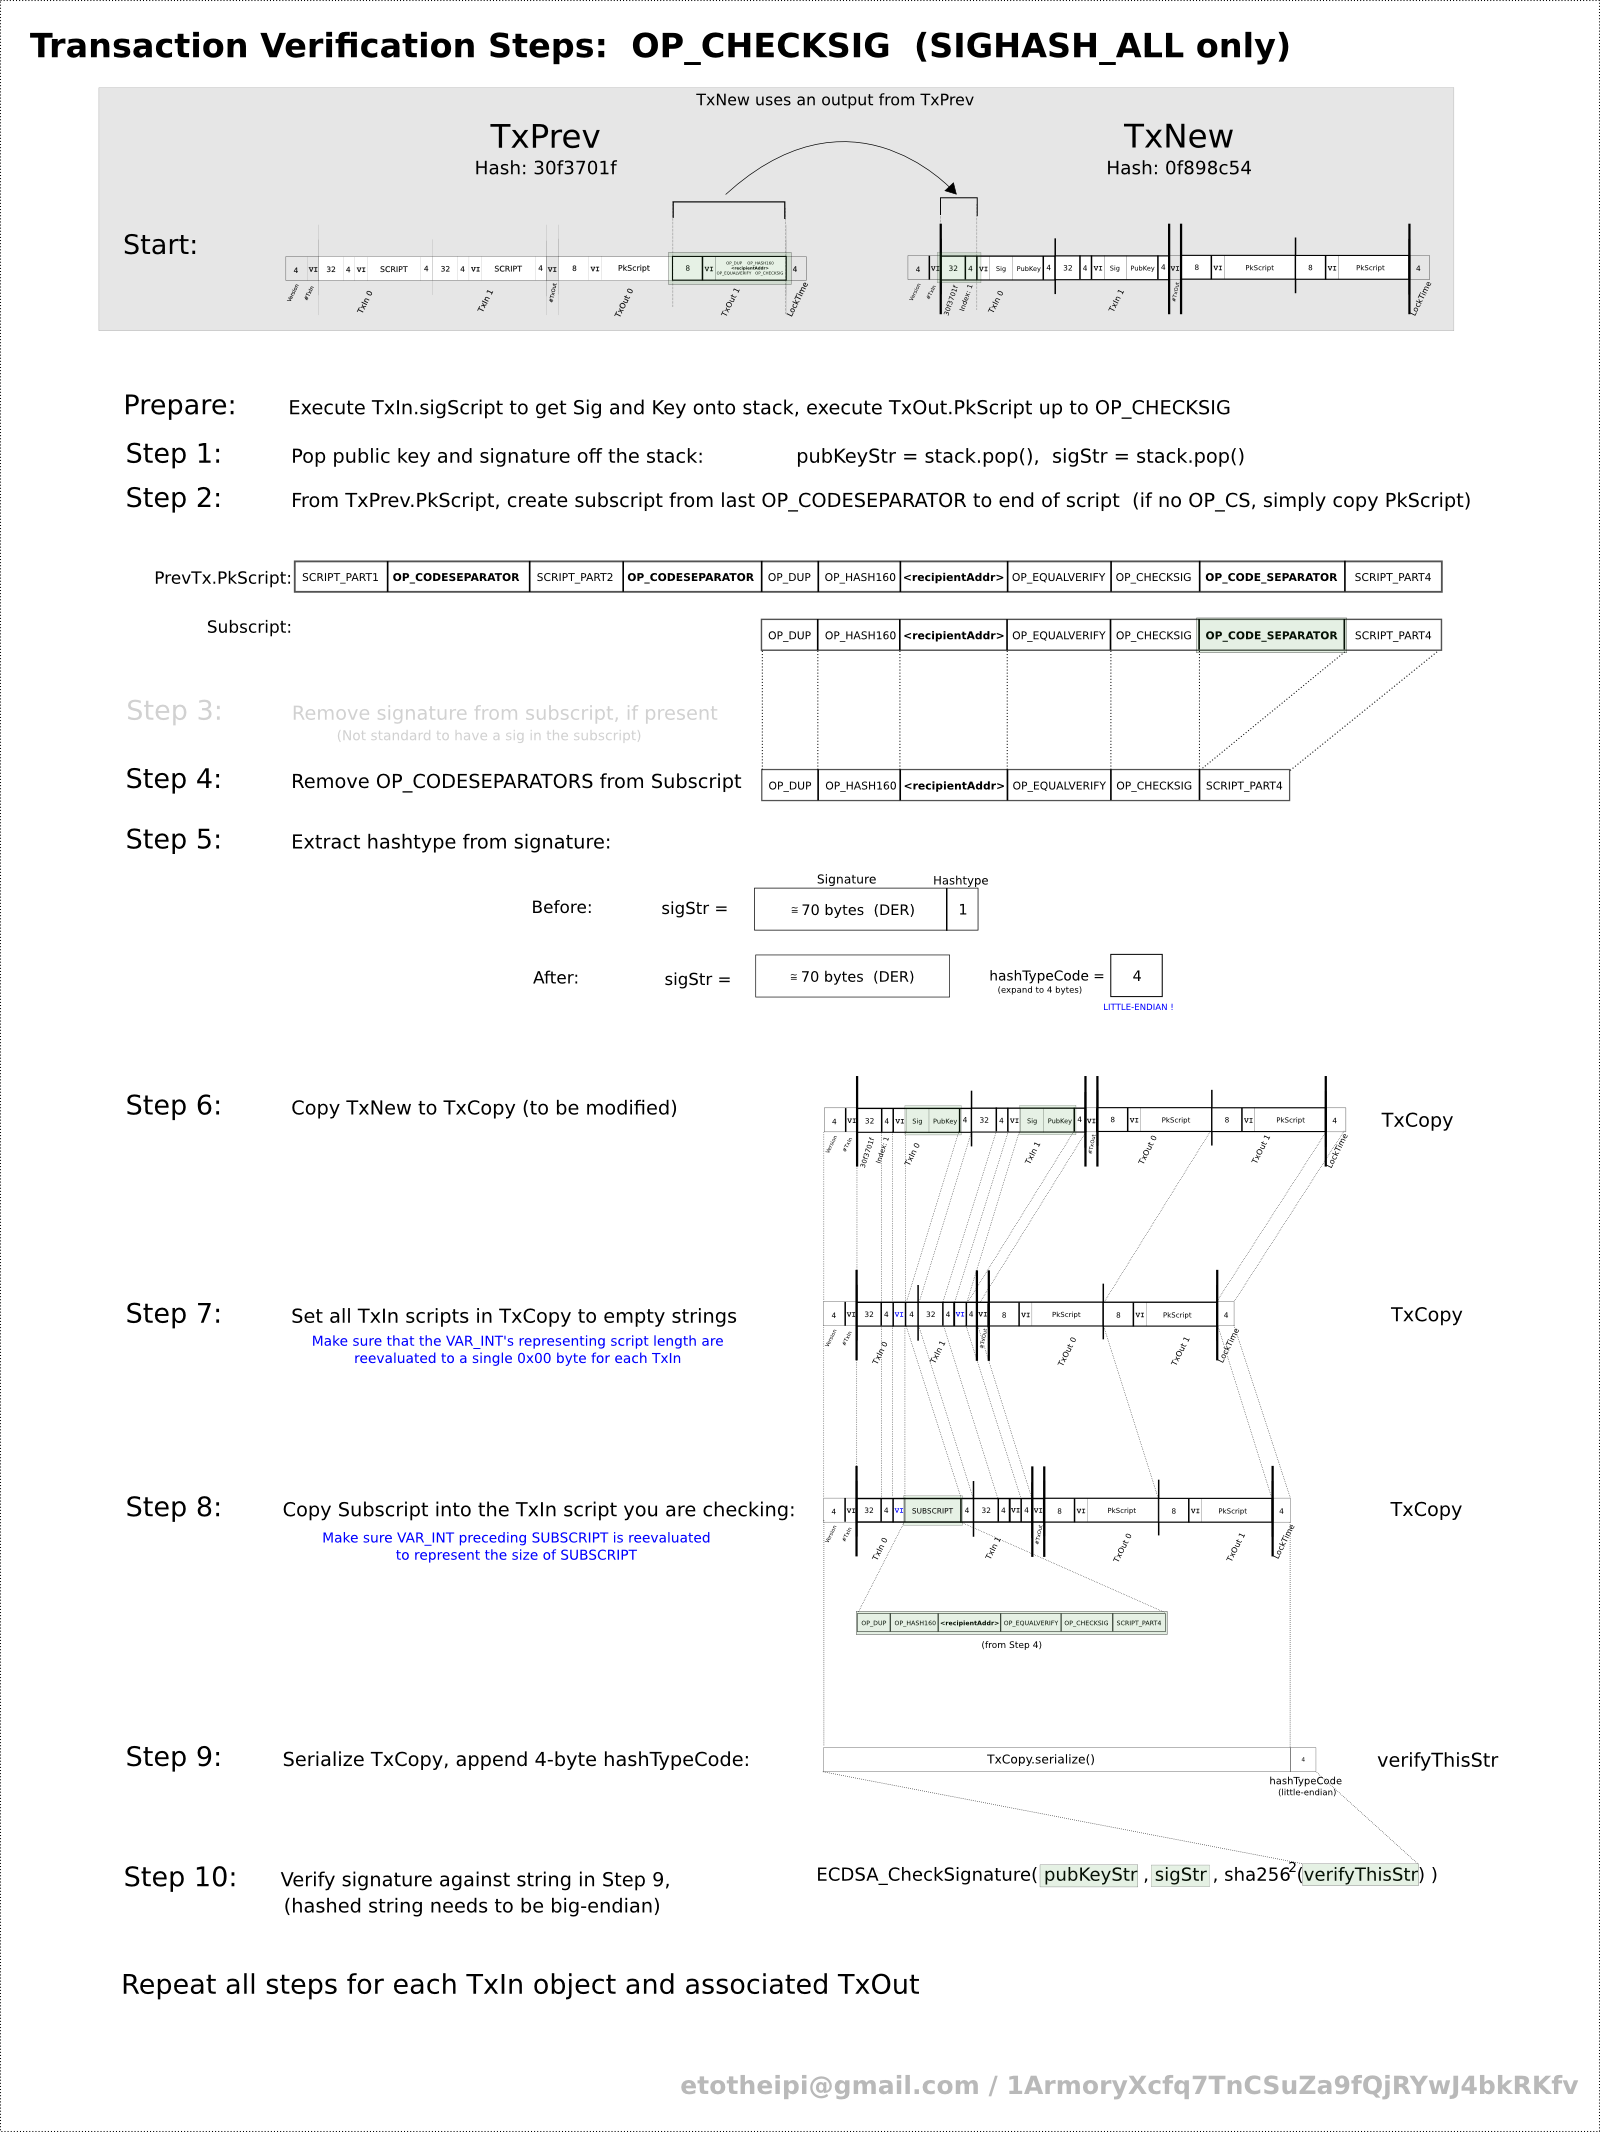
\includegraphics[width=1.35\textwidth]{background/images/checksig_in_detail.png}}
%\newpage

\Subsection{Pay to public key hash (P2PKH)}\label{p2pkh}
P2PKH is as mentioned the most common form of transaction.\cite{antonopoulos_2017} This transaction can be thought of as paying to somebodies address. In other words the output of this transaction contains a script where the one who wants to redeem it must prove that they own the private key which created the public key the address is referring too. This is what the script looks like in the output:

\texttt{OP\_DUP OP\_HASH160 <public key hash> OP\_EQUALVERIFY OP\_CHECKSIG}

As mentioned already executing the script in the output by it self doesn't make any sense, especially now when the very first operation \texttt{OP\_DUP} tries to duplicate the top element in the stack. But at execution the stack will be empty. Anyone wanting to spend this output would construct a transaction with the input script on the following form:

\texttt{<signature> <public key>}

When the input and output is executed together the process goes like this: 
\begin{enumerate}
	\item First the signature and unhashed public key is pushed to the stack.
	\item The public key is duplicated (there are now one signature and two public keys on the stack).
	\item The top public key goes through the HASH160 process making it a hashed public key.
	\item The hashed public key from the output is pushed on the stack, at this point the stack has the following elements (\texttt{<signature>}, \texttt{<public key>}, \texttt{<hashed public key>}, \texttt{<hashed public key>}).
	\item \texttt{OP\_EQUALVERIFY} checks if the top two elements is equal and verifies the result, What basically has been done is is that the script checks if the public key provided in the input script is equal to the hashed public key given in the output script.
	\item At this point the stack has the following elements: (\texttt{<signature>}, \texttt{<public key>}). \texttt{OP\_CHECKSIG} pops these from the stack and checks if the signature is valid.
\end{enumerate}

In the early days of bitcoin you payed directly to public keys instead of hashed public key. The reason the hash part was added at all has to do with extra security. If an exploit is found in elliptic curve cryptography that makes it so someone could calculate the private key from a public key then all unspent outputs would be at risk of being stolen. With the hashed public key the actual public key is not revealed until the output is spent, and then it is too late for it to be stolen. This of course requires that everyone uses a different public key for every transaction, which is the standard today.\cite{bitcoin_core_tx}

\Subsection{Pay to script hash (P2SH)}
Pay to script hash is slightly newer and a bit more complex to understand. Instead of paying to someones address, you pay to a script, this was initially proposed by Gavin Andreasen in 2012.\cite{scripthash} Let's say Alice has partial script S, that can be solved with the partial script K. She can then hash S and get $H_S$. She then creates transaction with an output containing the following script:

\texttt{OP\_HASH160 <$H_S$> OP\_EQUAL}

If Bob wants to redeem this transaction he first has to know the script and how to solve it. This is how the transaction input would look like: 

\texttt{K <S>}

The execution of the combined input output script is not straight forward as most scripts are. This is the process:
\begin{enumerate}
	\item The K part of the script is executed as usual. This pushes or does whatever it needs to do to make K + S a valid script.
	\item The partial script S is pushed to the stack in the form of bytes.
	\item This is where the execution takes a strange and not so intuitive path, as you will see. First the script is hashed with the \texttt{OP\_HASH160} operation.
	\item The script hash from the output is pushed on the stack.
	\item OP\_EQUAL checks if the top two items on the stack are equal. If they are it means that the script S provided in the input is the correct script.
	\item Unique to P2SH, the execution goes back to the original script S that was pushed to the stack in stage 2. And executes it together with whatever K pushed to the stack. This script also has to be valid.\cite{scripthash} 
\end{enumerate}

If all stages are executed without error the redeeming transaction is valid. 

P2SH was developed to resolve the difficulties in making complex transaction scripts and make them as simple as paying to an address. What P2SH basically means is ''pay to a script matching this hash, a script that will be presented later when this output is spent''\cite{antonopoulos_2017}\cite{scripthash}

\Subsection{Timelock and sequence}
Since the start of bitcoin; transactions has had two fields in them called \textbf{nTimelock} and \textbf{nSequence}. The timelock variable stopped a transaction from being  included in a block until a certain unix-timestamp or a certain blockheight\footnote{Blockheight is the number of blocks on the current chain} had passed. The sequence field is part of each input into a transaction, it's original purpose was to give users a mechanism for updating a transaction that were still in the transaction-pool. Miners were supposed to include the transaction version with highest sequence number, this however was unenforceable, as there is no way of knowing which transactions were in the transaction-pool of the miner at the time of block creation. So nSequence became mostly defunct and saw little use.

To make timelocks more versatile and more easily enforceable Peter Todd proposed an addition to Script, a new op-code that verifies that the correct timestamp is set, \\\texttt{OP\_CHECKTIMELOCKVERIFY}.

As timelocks only allows for absolute wait time, like for example: ''this transaction can only be spent after \texttt{10th June 2019}''. Mark Friedenbach et al. proposed in 2015 to add an additonal op code to Script that can check for relative time passage as well, \texttt{OP\_CHECKSEQUENCEVERIFY}.

\Subsubsection{OP\_CHECKTIMELOCKVERIFY}
There is an operation in Script called \texttt{OP\_CHECKTIMELOCKVERIFY}, what it does is that it compares the timestamp or blockheight that is on the stack and compares it to the timestamp that is in the transaction trying to spend the output that this op code is part of.\cite{antonopoulos_2017}\cite{checklocktime}\cite{script_wiki}\cite{bitcoin_core_tx}

\Subsubsection{OP\_CHECKSEQUENCEVERIFY}
\texttt{OP\_CHECKSEQUENCEVERIFY} is a lot like the previous one except it it deals with relative time. 

Let's say you have two transactions transaction $T_A$ and transaction $T_B$, $T_A$ is included in a block on the blockchain. If $T_B$ tries to spend one of $T_A$ outputs and has that specific input marked with a  sequence of 10. It means that $T_B$ can't be included in the block chain until $T_A$ is at least 10 blocks deep in the blockchain.\cite{antonopoulos_2017}\cite{checksequence}\cite{script_wiki}\cite{bitcoin_core_tx}

\texttt{OP\_CHECKSEQUENCEVERIFY} enforces this in the output. If $T_A$ has \texttt{10 OP\_CHECKSEQUENCEVERIFY}, then if $T_B$ tries to spend that output it has to be at least 10 blocks deep.


\Section{Payment channels}
A payment channel is a channel where transactions can be exchanged trustlessly on channels other than directly on the blockchain.
This is what is usually referred to as off-chain transactions.
In their most naive form a payment channel can simply be Alice and Bob exchanging promises of future transactions later.
This however is not trustless and any of the parties could later withdraw from the promise without punishment (other than maybe loss of friendship and future trust).

To build a trustless payment channel there are several ways to go about as Script is quite versatile.
The method that will be covered here uses a type of channel \textbf{funding transaction that requires the signature from both parties to spend}, and the channel balance is updated via special commitment transactions that spend the funding output. Each party in the channel has their own version of the commitment transaction. Whenever a commitment transaction is broadcast to the blockchain the channel is closed as the funding transaction can't be spent twice. To update the balance in the channel both parties create new commitment transactions and signs the other parties commitment transaction.\cite{lightningnetwork_2019}\cite{antonopoulos_2017}
Let's take a look at a naive example:

\Subsection{The naive payment channel}
Imagine Alice and Bob wants to open a payment channel between each other. They create a funding transaction and the initial commitment transactions. Let's say they both funded the channel with 1 Bitcoin each. The initial commitment transactions would then have one output paying 1 Bitcoin to Alice and one output paying 1 Bitcoin to Bob, let's call this commit (\textbf{C0}).
The funding transaction is broadcast to the blockchain.

A bit later Alice buys one funny hat from Bob for 0.1 Bitcoins. To complete the transaction they create two new commitment transaction that pays 0.9 Bitcoin to Alice and 1.1 Bitcoin to Bob and signs them for each other, let's call this new commitment (\textbf{C1}). Any number of transactions could be exchanged this way. The channel could be closed by any one broadcasting their commitment transaction. This naive implementation of a payment channel has a fatal flaw however. 

A payment channel needs some safety measures to be safe from malicious actors. The above example lacks a mechanism for preventing old commitment transactions from making their way into the blockchain and still paying the malicious party.. For example after the initial funny hat transaction above (\textbf{C1}) Alice could just broadcast the initial commit transaction (\textbf{C0}) and reclaim the 0.1 Bitcoins she spent. Bob would have no way of preventing this in this naive implementation.

\Subsection{Transaction flow diagrams}
The transactions that are involved in making payment channels grows larger the more features that are added. To make it easier to understand, diagrams are used together with the descriptions. In Figure \ref{fig:anatomy} a basic overview of the diagram-realm transaction is shown. Lines leading from outputs to inputs means that the connected input are spending that output. Note that one output can be connected to several inputs but each input can only be connected to one output, of course an output can only be spent once, this will be clarified later. A question mark (\textbf{?}) in the broadcaster field indicates either that the sender is unknown or that who sends it is irrelevant. 


\begin{figure}[H]
	\centering
	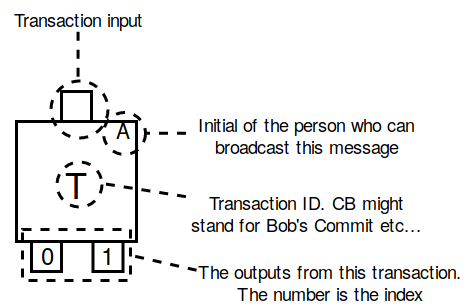
\includegraphics[width=0.5\textwidth]{background/images/tx_anatomy.png}
	\caption{Different parts of a transaction as they appear in diagrams.}
	\label{fig:anatomy}
\end{figure}

\Subsubsection{Payment channel with breach remedy}\label{breach_remedy}
To prevent old transactions from being sent to the blockchain a new mechanism needs to be devised. This can be done via something called revocable delivery and breach remedy (Some times called just revocation).
Instead of both parties holding the same commit. They each get an individual one that differs in its outputs. 

\begin{figure}[H]
	\centering
	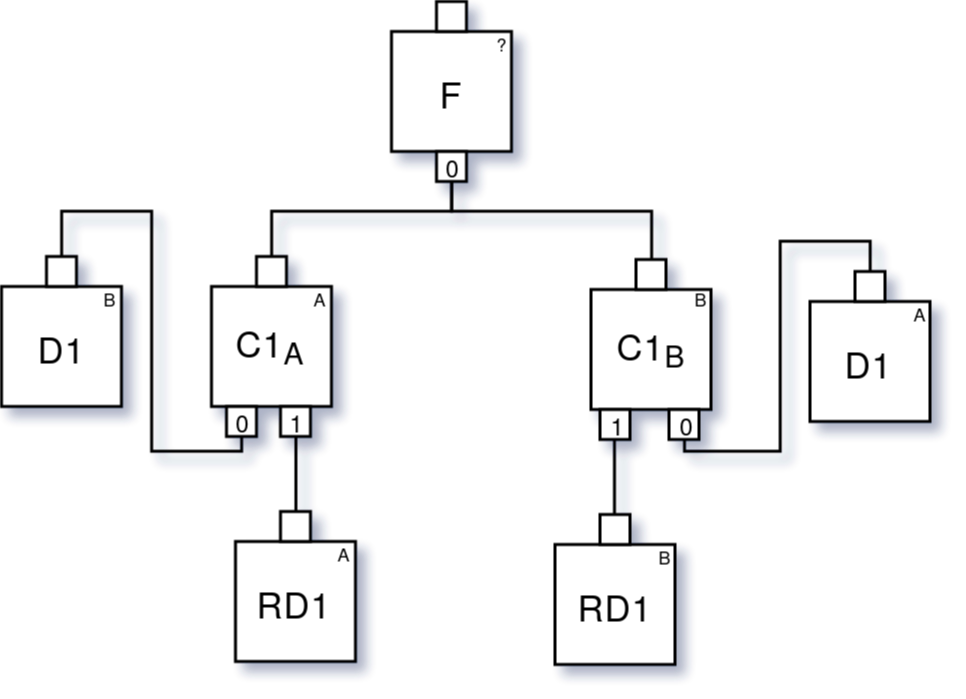
\includegraphics[width=0.6\textwidth]{background/images/payment_channel_pre_breach.png}
	\caption{Payment channel, with commits using revocable delivery mechanism}
	\label{fig:pre-breach}
\end{figure}

Figure \ref{fig:pre-breach} shows how the payment channel appears after the first commitment transactions has been made. Let's say the channel is between Alice (A) and Bob (B) and the balance in the channel is 0.5 BTC for Alice and 0.5 BTC for Bob. 

Let us take a look at the left side of this diagram. \textbf{$C1_{A}$} is the commitment transaction on Alice's side of the channel. As with all commitment transactions it spends the funding transaction. It has two outputs. Output 0 sends 0.5 BTC to Bob completely unencumbered. Output 1 is a bit more complicated however. It pays into a revocable delivery contract worth 0.5 BTC.\footnote{The contract is a script, and it is payed to via P2SH} The contract is constructed with a relative time lock that allows Alice to claim her share of the money after x amount of time (relative to the broadcast time of $C1_{A}$, often described in terms of blocks) or pays to whomever can sign using the pre-generated revocation keys (See section \ref{homomorphism})

D1 is the transaction Bob uses to claim his money in case Alice decides to broadcast her commitment transaction ($C1_{A}$).

RD1 is the transaction that Alice uses to claim her money. The transaction has a relative timelock on it that makes it so it can't be broadcast until x blocks has passed since $C1_{A}$ was included in the blockchain. \textbf{From now on the relative timelock will be 100 blocks in all the following examples}.

The right side is identical, only that the RD1 and D1 relationship is reversed, meaning that Alice can claim her money directly and Bob has to wait. 

If Alice wants to send 0.1 BTC to Bob they need to update the channel with new commitment transactions and then invalidate the old transaction. The transaction diagram will now look like figure \ref{fig:pc-update}

\begin{figure}[H]
	\centering
	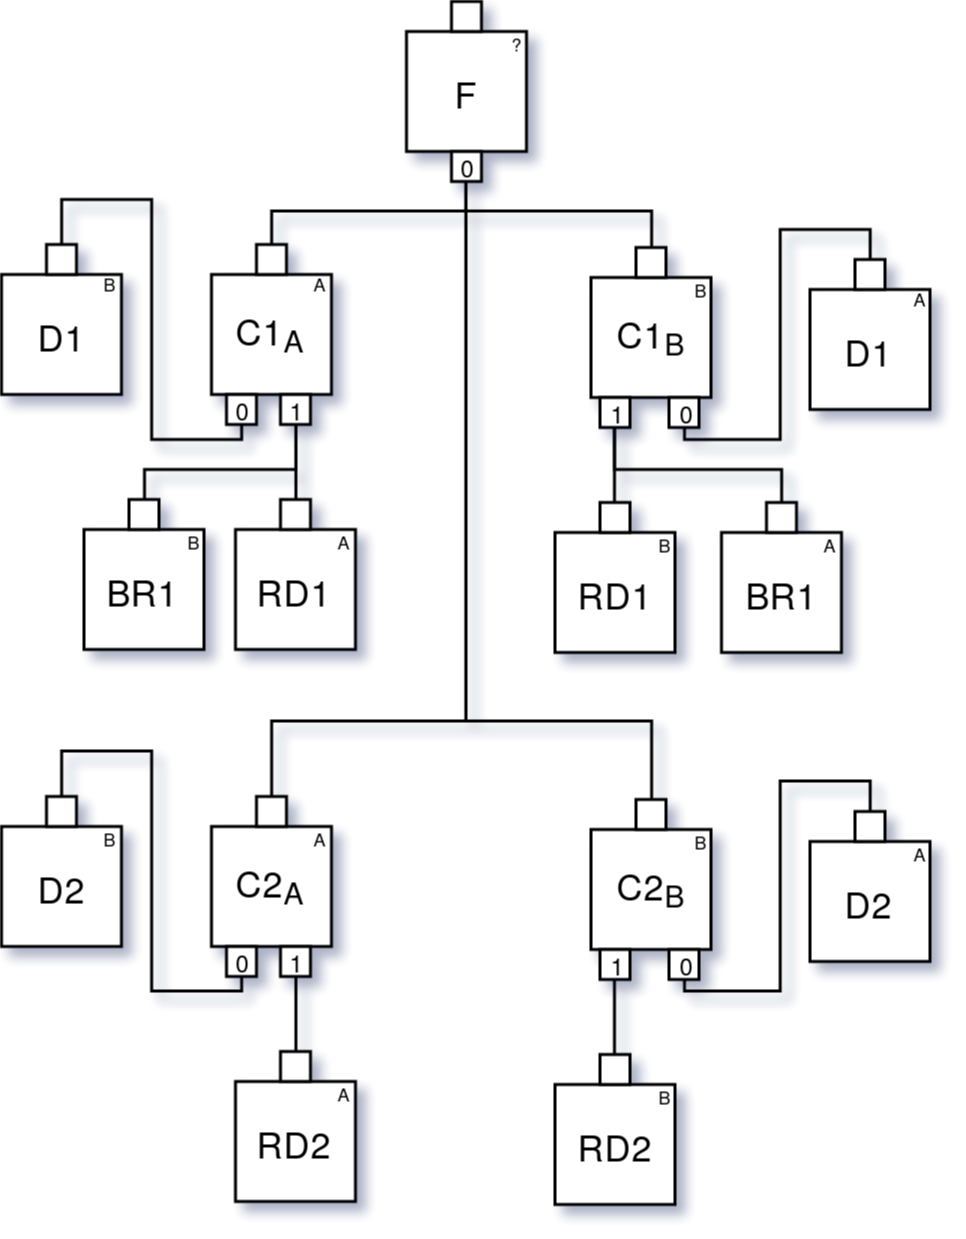
\includegraphics[width=0.65\textwidth]{background/images/payment_channel_updated.png}
	\caption{Updated payment channel, with breach remedies for old commitment transactions}
	\label{fig:pc-update}
\end{figure}

Figure \ref{fig:pc-update} shows the state of the channel after the new commitment transactions have been finalized. 
$C2_{A}$ is a lot like the previous commitment transaction with a few changes. The primary change is of course the channel balance, output 0 now has 0.6 BTC as value and output 1 has 0.4 BTC (Because Alice sent 0.1 BTC to Bob).

Another important update to the channel is the breach remedy. BR1 is the breach remedy for the first commitment transaction, its purpose is to prevent old commitment transactions from being broadcast.\cite{lightningnetwork_2019} The breach remedy can be created after Alice has revealed the secret private key she used when creating the revocation key. Of course to prevent a new false breach remedy to be created for $C2_{A}$ Alice uses a new revocation key for all new commitment transactions. If Alice tries to take back her money by broadcasting an old commitment transaction Bob can prevent it by broadcasting the breach remedy, this is possible because of the timelock on Alice's claim being time-locked.\cite{lightningnetwork_2019}

These are the steps taken whenever someone wants to send money in the channel (Under the assumption that commitment n-1 ($C_{n-1}$) was the latest commitment transaction in the channel), Alice is assumed to be the sender:\\\\
%\begin{enumerate}
	\textbf{1.} Both parties create new revocation public keys.\\
	\textbf{2.} Alice creates the commitment on Bob's side ($Cn_{b}$) using the revocation key from the previous step, signs it and sends it to Bob.\\
	\textbf{3.} Bob creates the commitment on Alice's side ($Cn_{a}$) using the revocation key from the previous step, signs it and sends it to Alice.\\
	\textbf{4.} Each party generates their respective Delivery and Revocable delivery transactions (Dn and BRn)\\
	\textbf{5.} Both parties reveal the secret used to create the revocation keys for the previous commitment transactions ($C_{n-1}$)\\
	\textbf{6.} From these revocation keys each party constructs the breach remedy ($BR_{n-1}$) for the previous commitment on the other persons side.\\
%\end{enumerate}

These steps can be repeated however many times until the channel is closed. 


\Section{Lightning network}
The payment channel I just described allows for unlimited transaction between two people.
It is quite usefull if you have two people who make a lot of transaction between each other,
but it would be very encumbersome to have a channel open to every person you might ever
make transactions to. This is where lightning network becomes useful. With just a few
additions to the payment channel it ill allow for transactions that travel through
multiple channels, safely of course.

To do this channels add another output to their commitment transactions that pay
to something called Hashed timelocked contract or HTLC for short. Just as before
I would like to cover the fine details of the contract, but there is no time for 
that. In simplest possible terms the contract says that each node along the way will
receive the money they put up plus a small fee if they can prove that the transaction
reached it's destination. This is done via hashes and pre-images, something I will touch
upon a bit later in this presentation.

The contract has a built in timelimit, if the transaction never makes it the whole way
to it's destination all transactions along the way will be refunded and nobody will receive
their fee. 

*Show basic image, talk about how large the network is* 
